\section{ĐƯỜNG TRÒN TRONG MẶT PHẲNG TỌA ĐỘ}
\subsection{LÝ THUYẾT CẦN NHỚ}
\subsubsection{Phương trình đường tròn có tâm và bán kính cho trước}
\immini{Trong mặt phẳng $Oxy$, đường tròn $\mathscr{(C)}\colon \heva{& \text{ tâm } I(a;b) \quad(1)\\& \text{ bán kính } R \quad(2)}$ có phương trình 
	\boxmini{$(x-a)^2+(y-b)^2=R^2 \quad(\star)$}
}{\hspace{1cm}
	\begin{tikzpicture}[scale=0.8]
		\tikzset{label style/.style={font=\footnotesize}}
		\tkzDefPoints{0/0/I,2/0/M}
		\tkzDrawCircle[radius](I,M)
		\tkzLabelPoints[below](I)
		\tkzLabelPoints[right](M)
		\tkzDrawPoints[size=3,fill=black](I,M)
		\tkzDrawSegments(I,M)
		\tkzLabelSegment[pos=0.5,below](I,M){$R$}
\end{tikzpicture}}
\subsubsection{Dạng khai triển}
\begin{itemize}
	\item [\iconMT] \indam{Phương trình đường tròn:}  Ta có thể khai triển $(\star)$, biến đổi phương trình về dạng 
	\boxmini{$x^2+y^2-2ax-2by+c=0 \quad (\star \star)$}
	trong đó $c=a^2+b^2-R^2$.
	\item [\iconMT] \indam{Chú ý:}
	\begin{gachsoc}
		\begin{itemize}
			\item [\ding{172}] Trong trường hợp tổng quát, điều kiện để $(\star \star)$ là phương trình đường tròn là $a^2+b^2-c>0$.
			\item [\ding{173}] Để xác định tâm và bán kính của đường tròn ở dạng $(\star \star)$, ta làm như sau:
			\begin{itemize}
				\item Đổi dấu hệ số trước $x$ và $y$ rồi chia 2, ta được tâm $I(a;b)$.
				\item Tính bán kính theo công thức $R=\sqrt{a^2+b^2-c}$. 
			\end{itemize}
		\end{itemize}
	\end{gachsoc}
\end{itemize}

\subsubsection{Phương trình tiếp tuyến của đường tròn}
\begin{itemize}
	\immini{\item [\iconMT] \indam{Công thức tiếp tuyến:} Cho đường tròn $\mathscr{(C)}$ có tâm $I(a;b)$ và bán kính $R$. Đường thẳng $\Delta $ là tiếp tuyến với $\mathscr{(C)}$ tại điểm $M_0\left(x_0;y_0\right)$. Khi đó
		\begin{itemize}
			\item [$\bullet$] $M_0\left(x_0;y_0\right)$ thuộc $\Delta $.
			\item [$\bullet$] $\overrightarrow{IM}_0=(x_0-a;y_0-b)$ là véc-tơ pháp tuyến của $\Delta $.
		\end{itemize}
		Do đó $\Delta $ có phương trình là
		\boxmini{$\left(x_0-a\right)\left(x-x_0\right)+\left(y_0-b\right)\left(y-y_0\right)=0.$}
	}{\vspace{1cm}\hspace{1cm}
		\begin{tikzpicture}[scale=0.7, font=\footnotesize, line join=round, line cap=round, >=stealth]
			\tkzDefPoints{0/0/I,-2/1/M_0}
			\clip (-3.5,-2.3) rectangle (2.5,2.6);
			\draw[->] (I)--(M_0);
			\tkzDrawCircle[radius](I,M_0)
			\tkzDefPointBy[rotation=center M_0 angle 90](I)\tkzGetPoint{M'}
			\tkzDefPointBy[rotation=center M_0 angle -90](I)\tkzGetPoint{M''}	
			\draw (M')--(M'');
			\node at (-3.2,-1) [above]{$\Delta$};
			\tkzDrawPoints[fill=black,size=3](I,M_0)
			\tkzLabelPoints[above left](M_0)
			\tkzLabelPoints[below](I)
		\end{tikzpicture}
	}
	\item [\iconMT] \indam{Chú ý:} Đường thẳng $\Delta$ tiếp xúc $\mathscr{(C)}$ khi $\mathrm{d}(I,\Delta)=R$.
\end{itemize}



\subsection{PHÂN LOẠI VÀ PHƯƠNG PHÁP GIẢI TOÁN}
\begin{dang}{Tìm tâm và bán kính đường tròn.}
	\begin{itemize}
		\item [\iconMT] \indam{Xét dạng $(x-a)^2+(y-b)^2=m\quad(1)$.}
		\begin{itemize}
			\item [\ding{172}] Nếu $m > 0$ thì (1) là phương trình đường tròn có tâm $I\left(a;b\right)$ và bán kính $R=\sqrt{m}$.
			\item [\ding{173}] Nếu $m\le 0$ thì (1) không phải là phương trình đường tròn.
		\end{itemize}
		\item [\iconMT] \indam{Xét dạng $x^2+y^2-2ax-2by+c=0 \quad(2)$.} Xét dấu biểu thức $m=a^2+b^2-c$.
		\begin{itemize}
			\item [\ding{172}] Nếu $m > 0$ thì (2) là phương trình đường tròn có
			\begin{itemize}
				\item  tâm $I\left(a;b\right)$;
				\item  bán kính $R=\sqrt{a^2+b^2-c}$.
			\end{itemize}
			\item [\ding{173}] Nếu $m\le 0$ thì (2) không phải là phương trình đường tròn.
		\end{itemize}
	\end{itemize}
\end{dang}

\begin{vd}
	Trong mặt phẳng $Oxy$, Tìm tâm và bán kính của đường tròn có phương trình sau đây.
	\begin{tasks}(2)
		\task $(x-1)^2+(y+2)^2=16$.
		\task $(x+2)^2+(y-3)^2=9$.
		\task $(x+2)^2+y^2=4$.
		\task $x^2+y^2=5$.
	\end{tasks}
	\loigiai{
		
	}
\end{vd}\dongcham{9}

\begin{vd}%[10EX- Tex hóa CD -CT-hk2-Thầy Trịnh Xuân]%[0H3Y2-1]
	Phương trình nào trong các phương trình sau đây là phương trình đường tròn? Tìm tọa độ tâm và bán kính của đường tròn đó.
	\begin{enumEX}{2}%số cột
		\item $x^2 + y^2 -2x-4y-20=0$;
		\item $x^2 + y^2+2x-4y+6=0$;
		\item $x^2 + y^2-4x-8y+5=0$;
		\item $2x^2 + 2y^2+6x+8y-2=0$.
	\end{enumEX}
	\loigiai{
		\begin{enumEX}{1}%số cột
			\item 
			$$	x^2 + y^2 -2x-4y-20=0\quad (1)$$			
			Phương trình $(1)$ có dạng $x^2 +y^2 -2ax -2by +c=0$ với $a= 1$; $b=2$; $c=-20$\\
			Ta có $a^2 + b^2 -c = 1+4+20 = 25>0$.\\
			Vậy $(1)$ là phương trình đường tròn có tâm $I(1;2)$ và có bán kính $R=5$.
			\item 
			$$x^2 + y^2+2x-4y+6=0\quad (2)$$
			Phương trình $(2)$ có dạng $x^2 +y^2 -2ax -2by +c=0$ với $a= -1$; $b=2$; $c=6$\\
			Ta có $a^2 + b^2 -c =1+4-6=-1<0$.\\
			Vậy $(2)$ không phải là phương trình đường tròn.
			\item 
			$$x^2 + y^2-4x-8y+5=0\quad (3)$$
			Phương trình $(3)$ có dạng $x^2 +y^2 -2ax -2by +c=0$ với $a= 2$; $b=4$; $c=5$\\
			Ta có $a^2 + b^2 -c =4+16-5=15>0$.\\
			Vậy $(2)$ là phương trình đường tròn tâm $I(2;4)$ và bán kính $R=\sqrt{15}$.
			\item 
			$$2x^2 + 2y^2+6x+8y-2=0
			\Leftrightarrow x^2 +y^2 +3x+4y-1=0\quad (4)$$	
			Phương trình $(4)$ có dạng $x^2 +y^2 -2ax -2by +c=0$ với $a= -\dfrac{3}{2}$; $b=-2$; $c=-1$\\
			Ta có $a^2 + b^2 -c =\dfrac{9}{4}+4+1=\dfrac{29}{4}>0$.\\
			Vậy $(4)$ là phương trình đường tròn tâm $I(-\dfrac{3}{2};-2)$ và bán kính $R=\dfrac{\sqrt{29}}{2}$.
			
		\end{enumEX}
	}
\end{vd}\dongcham{10}

\begin{vd}
	Trong mặt phẳng $Oxy$, cho phương trình $~x^2+y^2-2mx-4(m-2)y+6-m=0 \quad(1)$. Tìm điều kiện của $m$ để (1) là phương trình đường tròn.
	\loigiai{
		Phương trình (1) là phương trình đường tròn khi và chỉ khi $a^2+b^2-c > 0$, với $a=m;b=2(m-2);c=6-m$.\\
		Hay $m^2+4(m-2)^2-6+m > 0\Leftrightarrow 5m^2-15m+10 > 0\Leftrightarrow \hoac{
			& m > 2 \\ 
			& m < 1 
		}$.
	}
\end{vd}\dongcham{7}

\begin{dang}{Lập phương trình đường tròn}
	\begin{itemize}
		\item [\iconMT] \indam{Hướng tiếp cận 1.}  Từ giả thiết, giải tìm tọa độ tâm và tính độ dài bán kính. Sau đó, viết phương trình của $\mathscr{(C)}$ theo công thức $(x-a)^2+(y-b)^2=R^2$.
		\begin{boxkn}
			\begin{itemize}
				\item [\ding{172}] $\mathscr{(C)}$ có tâm $I$ và đi qua điểm $M$, suy ra $R=IM=\sqrt{(x_M-x_I)^2+(y_M-y_I)^2}$.
				\item [\ding{173}] $\mathscr{(C)}$ tiếp xúc với đường thẳng $\Delta $ tại $A$, suy ra $\mathrm{d}\left(I;\Delta\right)=R=IA$.\\
				\hspace*{2cm}
				\begin{tikzpicture}[scale=1]
					\tikzset{label style/.style={font=\footnotesize}}
					\tkzDefPoints{0/0/I,1/0/M}
					\tkzDrawCircle[radius](I,M)
					\tkzLabelPoints[below](I)
					\tkzLabelPoints[right](M)
					\tkzDrawPoints[size=3,fill=black](I,M)
					\tkzDrawSegments(I,M)
					\tkzLabelSegment[pos=0.5,below](I,M){\scriptsize $R$}
				\end{tikzpicture}
				\hspace{2cm}
				\begin{tikzpicture}[scale=0.9]
					\tikzset{label style/.style={font=\footnotesize}}
					\tkzDefPoints{0/0/I,0/-1/A,-2/-1/H,2/-1/K}
					\tkzDrawCircle[radius](I,A)
					\tkzLabelPoints[below](A)
					\tkzLabelPoints[above](I)
					\tkzDrawPoints[size=3,fill=black](I,A)
					\tkzDrawSegments(I,A H,K)
					\tkzLabelSegment[pos=0.5,right](I,A){\scriptsize$R$}
					\tkzLabelSegment[pos=1,below](H,K){\scriptsize$\Delta$}
				\end{tikzpicture}
			\end{itemize}
		\end{boxkn}
		\item [\iconMT] \indam{Hướng tiếp cận 2.} Thường dùng cho bài toán lập phương trình đường tròn ngoại tiếp tam giác (qua ba điểm) hoặc qua hai điểm và có tâm thuộc đường thẳng $d$.
		\begin{itemize}
			\item Giả sử phương trình đường tròn $\mathscr{(C)}$ là $x^2+y^2-2ax-2by+c=0 $
			\item Từ điều kiện của đề bài, ta thiết lập hệ phương trình với ba ẩn là $a,b,c$. Giải hệ tìm $a,b,c$.
		\end{itemize}
	\end{itemize}
\end{dang}
\begin{vd}
	Trong mặt phẳng $Oxy$, lập phương trình đường tròn $\mathscr{(C)}$, biết
	\begin{tasks}(2)
		\task $\mathscr{(C)}$  có tâm $I(3;-5)$ bán kính $R=2$.
		\task  $\mathscr{(C)}$ có tâm $I(3;-5)$ và qua điểm $A(-2;1)$.
	\end{tasks}
	
	\loigiai{
		
	}
\end{vd}\dongcham{13}
\begin{vd}
	Trong mặt phẳng $Oxy$, lập phương trình đường tròn đường kính $AB$ với $A\left(1;6\right)$, $B\left(-3;2\right)$.
	\loigiai{
		Đường tròn đường kính $AB$ có:
		\begin{itemize}
			\item Tâm $I\left(-1;4\right)$ là trung điểm $AB$.
			\item Bán kính $R=\dfrac{AB}{2}=2\sqrt{2}$.
		\end{itemize}
		Do đó phương trình đường tròn là:\\ $(x+1)^2+(y-4)^2=\left(2\sqrt{2}\right)^2\Leftrightarrow x^2+y^2+2x-8y+9=0$.
	}
\end{vd}\dongcham{10}
\begin{vd}
	Trong mặt phẳng $Oxy$, viết phương trình đường tròn $\mathscr{(C)}$ có tâm $I\left(-1;2\right)$ và tiếp xúc với đường thẳng $\Delta:x-2y+7=0$.
	\loigiai{
		Bán kính đường tròn $(C)$ chính là khoẳng cách từ $I$ tới đường thẳng $\Delta $ nên
		\begin{align*}
			R=\mathrm{d}\left(I;\Delta\right)=\dfrac{\left|-1-4-7\right|}{\sqrt{1+4}}=\dfrac{2}{\sqrt{5}}.
		\end{align*}
		Vậy phương trình đường tròn $(C)$ là: $(x+1)^2+(y-2)^2=\dfrac{4}{5}$.
	}
\end{vd}\dongcham{10}

\begin{vd}
	Trong mặt phẳng $Oxy$, lập phương trình đường tròn đi qua ba điểm $M\left(-2;4\right),N\left(5;5\right),P\left(6;-2\right)$.
	\loigiai{
		\begin{itemize}
			\item \textit{Cách 1.} Gọi phương trình đường tròn (C) có dạng là: $x^2+y^2-2ax-2by+c=0 $.\\
			Do đường tròn đi qua ba điểm $M,N,P$ nên ta có hệ phương trình:
			\begin{align*}
				\heva{
					4+16+4a-8b+c&=0 \\ 
					25+25-10a-10b+c&=0 \\ 
					36+4-12a+4b+c&=0}
				\Leftrightarrow \heva{
					& a=2 \\ 
					& b=1 \\ 
					& c=-20 }
			\end{align*} 
			Vậy phương trình đường tròn cần tìm là: $x^2+y^2-4x-2y-20=0 $.
			\item \textit{Cách 2.} Gọi $I\left(x;y\right)$ và $R$ là tâm và bán kính đường tròn cần tìm. Ta suy ra:
			\begin{align*}
				IM=IN=IP \Leftrightarrow \heva{
					&IM^2=IN^2 \\
					&IM^2=IP^2 }.
			\end{align*}
			nên ta có hệ 
			\begin{align*}
				\heva{
					&(x+2)^2+(y-4)^2=(x-5)^2+(y-5)^2 \\
					&(x+2)^2+(y-4)^2=(x-6)^2+(y+2)^2}
				\Leftrightarrow \heva{& x=2 \\
					& y=1}.
			\end{align*}
			Suy ra $I(2; 1)$, bán kính $IA=5$.\\
			Vậy phương trình đường tròn cần tìm $(C):(x-2)^2+(y-1)^2=25$.
		\end{itemize}
	}
\end{vd}\dongcham{14}

\begin{vd}
	Trong mặt phẳng tọa độ, một tín hiệu âm thanh phát đi từ một vị trí và được 3 thiết bị ghi tín hiệu đặt tại 3 vị trí $O(0 ; 0), A(1 ; 0), B(1 ; 3)$ nhận được cùng một thời điểm. Hãy xác định vị trí phát tín hiệu âm thanh.
	\loigiai{
		Gọi vị trí phát tín hiệu âm thanh là $I(a ; b)$.
		Do 3 thiết bị ghi tín hiệu đặt tại 3 vị trí $O, A, B$ nhận được cùng một thời điểm nên vị trí phát tín hiệu âm thanh phải cách đều 3 điềm $O, A, B$. Suy ra $I$ là tâm đường tròn $(C)$ ngoại tiếp tam giác $OAB$.\\
		Gọi $(C) \colon x^2+y^2-2ax-2by+c=0$. $(C)$ qua 3 điểm $O$, $A$, $B$ nên ta có hệ
		$$\heva{&c=0\\&1-2a=0\\&-2a-6b+10=0} \Leftrightarrow \heva{&a=\dfrac{1}{2}\\&b=\dfrac{3}{2}}$$
	}
\end{vd}\dongcham{11}
\begin{vd}
	Trong mặt phẳng $Oxy$, cho đường thẳng $d:2x-y-5=0$ và hai điểm $A\left(1;2\right), B\left(4;1\right)$. Viết phương trình đường tròn $\mathscr{(C)}$ có tâm thuộc $d$ và đi qua hai điểm $A, B$.
	\loigiai{
		\immini{
			\begin{itemize}
				
				\item \textit{Cách 1.} Gọi $I$ là tâm của $(C)$. Do $I\in d$ nên $I\left(t;2t-5\right)$.\\
				Hai điểm $A, B$ cùng thuộc $(C)$ nên 
				\begin{align*}
					IA=IB & \Leftrightarrow (1-t)^2+\left(7-2t\right)^2=(4-t)^2+\left(6-2t\right)^2\\
					& \Leftrightarrow t=1
				\end{align*}
				Suy ra $I(1;-3)$ và bán kính $R=IA=5$.\\
				Vậy phương trình đường tròn cần tìm là:
				\begin{align*}
					(C):(x-1)^2+(y+3)^2=25.
				\end{align*}
			\end{itemize}
		}
		{
			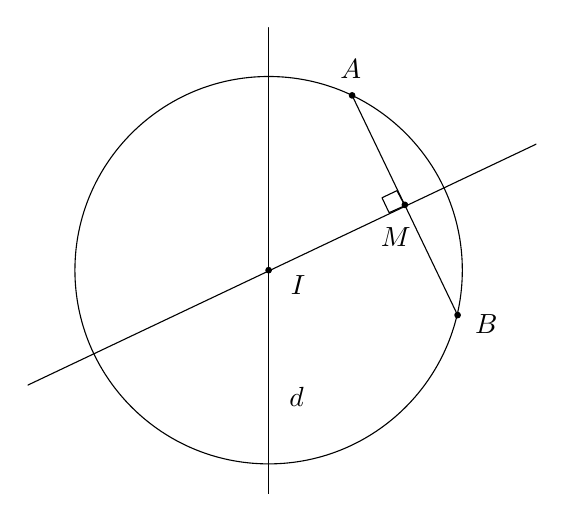
\begin{tikzpicture}[line cap=round,line join=round,>=stealth,x=1.0cm,y=1.0cm]
				\clip(1.24,-1.) rectangle (7.7,4.92);
				\draw (5.93,2.85) -- (5.74,2.76) -- (5.83,2.57) -- (6.03,2.66) -- cycle; 
				\draw (4.3,1.84) circle (2.46cm);
				\draw (5.36,4.06)-- (6.7,1.27);
				\draw [domain=1.24:7.7] plot(\x,{(-0.36--0.82*\x)/1.73});
				\draw (4.3,-1.) -- (4.3,4.92);
				\draw (5.6,4.4) node[left] {$A$};
				\draw (6.8,1.4) node[anchor=north west] {$B$};
				\draw (5.6,2.5) node[anchor=north west] {$M$};
				\draw (4.44,0.48) node[anchor=north west] {$d$};
				\draw (4.46,1.9) node[anchor=north west] {$I$};
				\draw [fill=black] (4.3,1.84) circle (1.0pt);
				\draw [fill=black] (5.36,4.06) circle (1.0pt);
				\draw [fill=black] (6.7,1.27) circle (1.0pt);
				\draw [fill=black] (6.03,2.67) circle (1.0pt);
			\end{tikzpicture}
		}
		\begin{itemize}
			\item \textit{Cách 2. }Gọi $M\left(\dfrac{5}{2};\dfrac{3}{2}\right)$ là trung điểm $AB$. Đường trung trực của đoạn $AB$ đi qua $M$ và nhận $\vec{AB}=(3;-1)$ làm vectơ pháp tuyến nên có phương trình $\Delta:3x-y-6=0$.\\
			Tọa độ tâm $I$ của $(C)$ là nghiệm của hệ $\heva{
				& 2x-y-5=0 \\ 
				& 3x-y-6=0 
			}\Rightarrow I(1;-3)$.\\
			Bán kính của đường tròn bằng $R=IA=5$.\\
			Vậy phương trình đường tròn cần tìm $(C):(x-1)^2+(y+3)^2=25$.
		\end{itemize}
	}
\end{vd}\dongcham{11}

\begin{vd}
	Trong mặt phẳng $Oxy$, cho đường thẳng $d\colon 2x-y-4=0$. Viết phương trình đường tròn $\mathscr{(C)}$ tiếp xúc với các trục tọa độ và có tâm ở trên đường thẳng $d$.
	\loigiai{
		Gọi $I(m;2m-4)\in d$ là tâm đường tròn $(C)$. Theo giả thiết bài toán, ta có
		$$\mathrm{d}(I,Ox)=\mathrm{d}(I,Oy) \Leftrightarrow |2m-4|=|m| \Leftrightarrow m=4\text{ hoặc }m=\dfrac{4}{3}.$$
		\begin{itemize}
			\item Với $m=\dfrac{4}{3}$, suy ra $I\left(\dfrac{4}{3};-\dfrac{4}{3}\right)$. Bán kính đường tròn $R=\mathrm{d}(I,Oy)=|m|=\dfrac{4}{3}$.\\
			Vậy phương trình đường tròn $(C)\colon \left(x-\dfrac{4}{3}\right)^2+\left(y+\dfrac{4}{3}\right)^2=\dfrac{16}{9}$.
			\item Với $m=4$, suy ra $I(4;4)$. Bán kính đường tròn $R=\mathrm{d}(I,Oy)=|m|=4$.\\
			Vậy phương trình đường tròn $(C)\colon (x-4)^2+(y+4)^2=16$.
		\end{itemize}
	}
\end{vd}\dongcham{11}

\begin{vd}
	Trong mặt phẳng $Oxy$, viết phương trình đường tròn $\mathscr{(C)}$ đi qua điểm $A(4;2)$ đồng thời tiếp xúc với hai đường thẳng $d_1 \colon x-3y-2=0$ và $d_2 \colon x-3y+18=0$.
	\loigiai{
		Gọi $I(a,b)$ và $R$ lần lượt là tâm và bán kính của $\mathscr{(C)}$. Ta có
		\begin{itemize}
			\item [$\bullet$] $\mathrm{d}(I,d_1)=\mathrm{d}(I,d_2) \Leftrightarrow \dfrac{\bigg|a-3b-2\bigg|}{\sqrt{10}}=\dfrac{\bigg|a-3b+18\bigg|}{\sqrt{10}} \Leftrightarrow a-3b+8=0 \Leftrightarrow a=3b-8\quad \quad (1)$
			\item [$\bullet$] $\mathrm{d}(I,d_1)=IA \Leftrightarrow \dfrac{\bigg|a-3b-2\bigg|}{\sqrt{10}}=\sqrt{(4-a)^2+(2-b)^2}\quad \quad (2)$.
		\end{itemize} 
		Thay (1) vào (2) và thu gọn, ta giải được $b=3$ hoặc $b=\dfrac{23}{5}$.
		\begin{itemize}
			\item [$\bullet$] Với $b=3$ thì $a=1$ và $R=\sqrt{10}$.
			\item [$\bullet$] Với $b=\dfrac{23}{5}$ thì $a=\dfrac{29}{5}$ và $R=\sqrt{10}$.
		\end{itemize}
		Vậy, có hai đường tròn $(x-1)^2+(y-3)^2=10$  hoặc $\left( x-\dfrac{29}{5}\right)^2+\left( y-\dfrac{23}{5}\right) ^2=10$. }
\end{vd}\dongcham{17}
\begin{dang}{Tiếp tuyến của đường tròn tại một điểm}
	\immini{
		Cho đường tròn $\mathscr{(C)}$ có tâm $I(a;b)$ và bán kính $R$. Đường thẳng $\Delta $ là tiếp tuyến với $\mathscr{(C)}$ tại điểm $M_0\left(x_0;y_0\right)$. Khi đó
		\begin{itemize}
			\item [$\bullet$] $M_0\left(x_0;y_0\right)$ thuộc $\Delta $.
			\item [$\bullet$] $\overrightarrow{IM}_0=(x_0-a;y_0-b)$ là véc-tơ pháp tuyến của $\Delta $.
		\end{itemize}
		Do đó $\Delta $ có phương trình là
		\begin{center}
			\fbox{$\left(x_0-a\right)\left(x-x_0\right)+\left(y_0-b\right)\left(y-y_0\right)=0.$}.
		\end{center}
	}{\hspace{1cm}
		\begin{tikzpicture}[scale=0.7, font=\footnotesize, line join=round, line cap=round, >=stealth]
			\tkzDefPoints{0/0/I,-2/1/M_0}
			\clip (-3.5,-2.3) rectangle (2.5,2.6);
			\draw[->] (I)--(M_0);
			\tkzDrawCircle[radius](I,M_0)
			\tkzDefPointBy[rotation=center M_0 angle 90](I)\tkzGetPoint{M'}
			\tkzDefPointBy[rotation=center M_0 angle -90](I)\tkzGetPoint{M''}	
			\draw (M')--(M'');
			\node at (-3.2,-1) [above]{$\Delta$};
			\tkzDrawPoints[fill=black,size=4](I,M_0)
			\tkzLabelPoints[above left](M_0)
			\tkzLabelPoints[below](I)
		\end{tikzpicture}
	}	
\end{dang}

\begin{vd}
	Trong mặt phẳng $Oxy$, viết phương trình tiếp tuyến của đường tròn $\mathscr{(C)} \colon  (x-2)^2+(y+3)^2=5$ tại điểm $M(3;-1)$.
	\loigiai{
		Đường tròn $(C)$ có tâm $I(2;-3)$.
		\\ Phương trình tiếp tuyến của $(C)$ tại điểm $M(3;-1)$ là: 
		\begin{align*}
			&(3-2)(x-3)+(-1+3)(y+1)=0 \\ \Leftrightarrow &x+2y-1=0.
		\end{align*}
		Vậy phương trình  tiếp tuyến của $(C)$ tại điểm $M(3;-1)$ là $ x+2y-1=0 $.
	}
\end{vd}\dongcham{10}

\begin{vd}%[0H3Y2-3]
	Viết phương trình tiếp tuyến $d$ với đường tròn $(C)\colon (x-1)^2+(y-3)^2=25$ tại điểm $M(5;6)$.
	\loigiai{
		Ta có $(5-1)^2+(6-3)^2=25$, nên điểm $M$ thuộc đường tròn $(C)$.\\
		Đường tròn $(C)\colon (x-1)^2+(y-3)^2=25$ có tâm $I(1;3)$.\\
		Phương trình tiếp tuyến $d$ với $(C)$ tại $M(5;6)$ là\\
		$$(1-5)(x-5)+3-6(y-6)=0\Leftrightarrow 4x+3y-38=0.$$
	}
\end{vd}\dongcham{7}

\begin{vd}%[0H3B2-3]
	Cho đường tròn $ (C)\colon x^2+y^2-8x-6y+17=0 $. Chứng minh $ M(6;5) $ nằm trên đường tròn $ (C) $. Viết phương trình tiếp tuyến $ d $ của $ (C) $ tại $ M $.
	%\dapso{$ x+y-11=0 $}
	\loigiai
	{
		Đường tròn $ (C)\heva{&\text{Tâm\,\,}I(4;3)\\&R=\sqrt{4^2+3^2-17}=2\sqrt{2}.} $\\
		Ta có $ 6^2+5^2-8\cdot 6-6\cdot 5+17=0 $ \quad(luôn đúng) $ \Rightarrow M\in (C) $.\\
		Ta lại có $ d \heva{&\text{qua\,\,}M(6;5)\\&\text{VTPT\,\,}\overrightarrow{IM}=(2;2).} $\\
		Phương trình tiếp tuyến $ d \colon x+y-11=0 $.
	}
\end{vd}\dongcham{7}

\begin{dang}{Tiếp tuyến của đường tròn song song hoặc vuông góc với một đường cho trước}
	Cho đường tròn $\mathscr{(C)}$ có tâm $I(a;b)$ và bán kính $R$.
	\begin{itemize}
		\item [\iconMT] \indam{Loại 1:} Biết tiếp tuyến song song với $d \colon Ax + By +C=0$.
		\begin{itemize}
			\item [$\bullet$] Gọi $\Delta$ là tiếp tuyến và $\Delta \parallel d$ nên $\Delta$ có dạng $Ax + By +m=0$, với $m \ne C$.
			\item [$\bullet$] $\Delta$ tiếp xúc $\mathscr{(C)}$ khi và chỉ khi
			$$\mathrm{d}(I,\Delta)=R \Leftrightarrow \dfrac{\bigg|A\cdot a+ B \cdot b +m\bigg|}{\sqrt{A^2+B^2}}=R$$ 
		\end{itemize}
		Giải điều kiện này, tìm $m$.
		\begin{luuy}
			Chú ý rằng $m$ phải khác $C$. Nếu giải ra giá trị $m=C$ thì ta loại giá trị này. 
		\end{luuy}
		\item [\iconMT] \indam{Loại 2:} Biết tiếp tuyến vuông góc với $d \colon Ax + By +C=0$.
		\begin{itemize}
			\item [$\bullet$] Gọi $\Delta$ là tiếp tuyến và $\Delta \perp d$ nên $\Delta$ có dạng $Bx - Ay +n=0$.
			\item [$\bullet$] $\Delta$ tiếp xúc $\mathscr{(C)}$ khi và chỉ khi
			$$\mathrm{d}(I,\Delta)=R \Leftrightarrow \dfrac{\bigg|B\cdot a-A \cdot b +n\bigg|}{\sqrt{A^2+B^2}}=R$$ 
		\end{itemize}
		Giải điều kiện này, tìm $n$.
	\end{itemize}
\end{dang}

\begin{vd}
	Trong mặt phẳng $Oxy$, cho đường tròn $\mathscr{(C)}: (x-1)^2+y^2=9$. Viết phương trình tiếp tuyến của đường tròn $\mathscr{(C)}$ biết rằng tiếp tuyến song song với đường thẳng $y=2x-1$.
	\loigiai{Gọi phương trình tiếp tuyến $(\Delta)$ song song với $y=2x-1$ là $y-2x+n=0$.
		\\ Đường tròn $(C)$ có tâm $I(1;0)$ và bán kính $R=3$.
		\\ Ta có \begin{align*}
			\mathrm{d}(I,\Delta)=\dfrac{|n-2|}{\sqrt{5}}=3 \Leftrightarrow \left[\begin{array}{ll}
				n=2-3\sqrt{5} \\ n=2+3\sqrt{5}.
			\end{array}\right.
		\end{align*}
		Phương trình tiếp tuyến $(\Delta)$ là $y-2x+2-3\sqrt{5}=0$ hoặc $y-2x+2+3\sqrt{5}=0$.}
\end{vd}\dongcham{11}

\begin{vd} %[0H3K2-3]%
	Cho đường tròn $(C) \colon x^2+y^2+2x-6y+5=0$. Viết phương trình tiếp tuyến của $(C)$ song song với đường thẳng
	$d:x+2y-15=0$.
	\loigiai{
		Ta có $(C) \colon (x+1)^2+(y-3)^2=5$, cho nên $(C)$  có tâm $I(-1;3)$ và bán kính $R=\sqrt{5}$. Đường thẳng $d'$ song song với $d$ có dạng $d' \colon x+2y+c=0, c \ne -15 $. Theo giả thiết $d'$ tiếp xúc với $(C)$ suy ra
		\[\mathrm{d} (I,d') = \sqrt{5} \Leftrightarrow \dfrac{|5+c|}{\sqrt{5}}=\sqrt{5}\Leftrightarrow \hoac{&c=0\\&c=-10}.\]
		Khi đó phương trình các tiếp tuyến là $x+2y=0; x+2y-10=0$.
	}
\end{vd}\dongcham{12}

\begin{vd}
	Trong mặt phẳng $Oxy$, viết phương trình tiếp tuyến $(\Delta)$ của đường tròn $\mathscr{(C)}\colon x^2+y^2-2x+4y+4=0$ biết rằng tiếp tuyến vuông góc với đường thẳng $x+2y+5=0$.
	\loigiai{Đường tròn $(C)$ có tâm $I(1;-2)$ và bán kính $R=1$.
		\\ Vì $\Delta$ vuông góc với đường thẳng $x+2y+5=0$ nên phương trình $\Delta$ có dạng $2x-y+m=0$.
		\\ Vì $\Delta$ là tiếp tuyến của $(C)$ nên ta có
		\begin{align*}
			\mathrm{d}(I,\Delta)=R & \Leftrightarrow \dfrac{|2+2+m|}{\sqrt{1^2+2^2}} =1 \\
			& \Leftrightarrow |4+m|=\sqrt{5} \\
			&\Leftrightarrow \left[ \begin{array}{ll}
				m=\sqrt{5}-4 \\ m=-\sqrt{5}-4.
			\end{array} \right.
		\end{align*}
		Nếu $m=\sqrt{5}-4$ thì phương trình của $\Delta$ là $2x-y+\sqrt{5}-4=0$.
		\\ Nếu $m=\-\sqrt{5}-4$ thì phương trình của $\Delta$ là $2x-y-\sqrt{5}-4=0$.
	}
\end{vd}\dongcham{12}

\begin{vd}%[0H3K2-3]%
	Trong mặt phẳng $Oxy$, cho đường tròn $(\mathrm{C}): x^2+y^2+4x+4y-17=0$. Viết phương trình tiếp tuyến $\Delta$ của  $(\mathrm{C})$ biết $\Delta$ vuông góc với đường thẳng $d\colon 3x-4y+1=0$.
	\loigiai{
		Đường tròn $(C)$ có tâm $I(-2;-2)$, bán kính $R=5$.\\
		$\Delta\perp d$ suy ra $\Delta\colon 4x+3y+c=0$.\\
		Ta có $\Delta$ là tiếp tuyến của đường tròn suy ra $$d(I,\Delta)=R\Leftrightarrow \dfrac{|4(-2)+3(-2)+c|}{\sqrt{4^2+3^2}}=5\Leftrightarrow |-14+c|=25\Leftrightarrow \hoac{&c=39\\ &c=-11.}$$
		Suy ra $\Delta\colon 4x+3y+39=0$ và $\Delta\colon 4x+3y-11=0$.
	}
\end{vd}\dongcham{12}

\subsection{BÀI TẬP TỰ LUYỆN}

\begin{baitap}%[0H3Y2-1]
	Phương trình nào sau đây là phương trình đường tròn?
	\begin{enumerate}
		\item $x^2+y^2-2x+2y-7=0$.
		\item $x^2+y^2-8x+2y+20=0$.
	\end{enumerate}
	\loigiai{
		\begin{enumerate}
			\item Ta có $a=1$, $b=-1$, $c=-7$ nên $a^2+b^2-c=1^2+(-1)^2-(-7)=9>0$.\\
			Do đó phương trình đã cho là phương trình đường tròn $(C)$ có tâm $I(1;-1)$, bán kính $R=\sqrt{9}=3$.
			\item Ta có $a=4$, $b=-1$, $c=20$ nên $a^2+b^2-c=4^2+(-1)^2-20=-3<0$.\\
			Do đó phương trình đã cho không là phương trình đường tròn.
		\end{enumerate}
	}
\end{baitap}\cham{8}
\begin{baitap}%[0H3Y2-1]
	Tìm tâm và bán kính của đường tròn trong mỗi trường hợp sau
	\begin{enumerate}
		\item Đường tròn có phương trình $(x+1)^2+(y-5)^2=9$.
		\item Đường tròn có phương trình $x^2+y^2-6x-2y-15=0$.
	\end{enumerate}
	\loigiai{
		\begin{enumerate}
			\item Đường tròn đã cho có tâm $I(-1;5)$, bán kính $R=3$.
			\item Ta có $a=3$, $b=1$, $c=-15$.\\
			Suy ra đường tròn đã cho có tâm $I(3;1)$, bán kính $R=\sqrt{3^2+1^2-(-15)}=5$.
		\end{enumerate}
	}
\end{baitap}\cham{9}

\begin{baitap} %[0H3Y2-2]%
	Viết Phương trình đường tròn có tâm $I(2;3)$ và bán kính $R=2$.
	\loigiai{Đường tròn $(C)$ có $\heva{&\text{tâm}\, I(2;3)\\&\text{bán kính} \ R=2.}$\\ nên phương trình đường tròn $(C)$ là: $(x-2)^2 +(y-3)^2=4$.
	}
\end{baitap}\cham{5}

\begin{baitap} %[0H3Y2-2]%
	Lập phương trình đường tròn $(C)$ trong các trường hợp sau:
	\begin{enumerate}[a)]
		\item $(C)$ có tâm $I(-2;3)$ và đi qua điểm $M(2;-3)$;
		\item $(C)$ có tâm $I(-1;2)$ và tiếp xúc với đường thẳng $\Delta \colon x-2y+7=0$;
		\item $(C)$ có đường kính $AB$ với $A(1;1)$ và $B(7;5)$.
	\end{enumerate}
	\loigiai{
		\begin{enumerate}[a)]
			\item Ta có: $IM^2=(2+2)^2+(-3-3)^2=52$.\\
			Phương trình đường tròn	$(C)$ có tâm $I(-2;3)$ với bán kính $R=IM$ là: $(x+2)^2 +(y-3)^2 =52$.
			\item Bán kính đường tròn chính bằng khoảng cách từ tâm $I$ đến đường thẳng $\Delta$ nên ta có: $R=\mathrm{d}(I;\Delta)= \dfrac{|-1-4+7|}{\sqrt{1+4}}=\dfrac{2}{\sqrt{5}}$. \\
			Vậy phương trình đường tròn $(C)$ cần tìm là $(x+1)^2 +(y-2)^2=\dfrac{4}{5}$.
			\item Gọi $I$ là trung điểm của $AB$. Khi đó tọa độ điểm $I$ là $I(4;3)$.\\
			Ta có: $IA^2=(4-1)^2 +(3-1)^2=13$.\\
			Phương trình đường tròn $(C)$ có tâm $I(4;3)$ và nhận $IA$ làm bán kính có phương trình là:
			
			\centering{$(x-4)^2 +(y-3)^2 =13$}.
		\end{enumerate}
	}
\end{baitap}\cham{20}

\begin{baitap}%[0H3K2-2]
	Lập phương trình đường tròn ngoại tiếp tam giác có tọa độ các đỉnh là:
	\begin{enumEX}{2}%số cột
		\item $A(1;4)$, $B(0;1)$,$C(4;3)$;
		\item $O(0;0)$, $P(16;0)$, $R(0;12)$.
	\end{enumEX}
	\loigiai{
		\begin{listEX}[]%số cột
			\item Gọi phương trình cần tìm là $(C)\colon x^2 +y^2 -2ax -2by+c=0$.\\
			Vì $(C)$ đi qua $A$, $B$, $C$ nên ta có hệ phương trình: $\heva{2a+8b-c&=17\\2b-c&=1\\8a+6b-c&=25}\Leftrightarrow\heva{&a=2\\&b=2\\&c=3.}$\\
			Vậy đường tròn $(C)$ có tâm $I(2;2)$ và bán kính $R=\sqrt{a^2+b^2-c}=\sqrt{2^2+2^2-3}=\sqrt{5}$.\\
			Phương trình đường tròn cần tìm là: $(x-2)^2+(y-2)^2=5$.
			\item 
			Gọi phương trình cần tìm là $(C)\colon x^2 +y^2 -2ax -2by+c=0$.\\
			Vì $(C)$ đi qua $O$, $P$, $R$ nên ta có hệ phương trình:$\heva{c&=0\\32a-c&=256\\24b-c&=144}\Leftrightarrow\heva{&a=8\\&b=6\\&c=0.}$\\
			Vậy đường tròn $(C)$ có tâm $I(8;6)$ và bán kính $R=\sqrt{a^2+b^2-c}=\sqrt{8^2+6^2-0}=10$.\\
			Phương trình đường tròn cần tìm là: $(x-8)^2+(y-6)^2=100$.
		\end{listEX}
	}
\end{baitap}\cham{22}

\begin{baitap}%[0H3B2-3]%
	Viết phương trình tiếp tuyến của đường tròn $(C)\colon x^2+y^2+4x+4y+3=0$ tại điểm $ M\left(-3;0\right) $.
	%\dapso{$ x-2y+3=0 $}
	\loigiai
	{
		Ta có đường tròn $ (C)\heva{&\text{Tâm\,\,}I(-2;-2)\\&R=\sqrt{(-2)^2+(-2)^2-3}=\sqrt{5}.} $.\\
		Gọi $ (\Delta) $ là phương trình tiếp tuyến cần tìm. Khi đó\\
		$ (\Delta)\heva{&\text{qua\,\,}M(-3;0)\\&\text{VTPT\,\,}\overrightarrow{IM}=(-1;2)} \Rightarrow$ phương trình $ (\Delta)\colon x-2y+3=0$.
	}
\end{baitap}\cham{10}


\begin{baitap}%[0H3B2-3]%
	Lập phương trình tiếp tuyến của đường tròn $ (C)\colon x^2+y^2-4x-2y=0 $ tại $ A $ có hoành độ là $ 0 $.
	\loigiai{
		Ta có đường tròn $ (C)\heva{&\text{Tâm\,\,}I(2;1)\\&R=\sqrt{2^2+1^2-0}=\sqrt{5}.} $.\\
		Gọi $ (\Delta) $ là phương trình tiếp tuyến cần tìm. Khi đó
		$ (\Delta)\heva{&\text{qua\,\,}A(0;y_A)\\&\text{VTPT\,\,}\overrightarrow{IA}.}$\\ Ta có $ x_A=0\Rightarrow  0^2+y_A^2-4\cdot 0-2y_A=0\Leftrightarrow \hoac{&y_A=0\Rightarrow \overrightarrow{IA}=(-2;-1)\Rightarrow (\Delta)\colon 2x+y=0\\&y_A=2\Rightarrow \overrightarrow{IA}=(-2;1)\Rightarrow (\Delta)\colon 2x-y+2=0}$.\\
		Vậy có hai phương trình tiếp tuyến cần tìm là $ 2x+y=0 $ và $ 2x-y+2=0 $.
	}
\end{baitap}\cham{10}


\begin{baitap}%[0H3B2-3]%
	Trong mặt phẳng tọa độ $Oxy$, cho đường tròn $(C)\colon x^2+y^2-6x+2y+5=0$. Viết phương trình tiếp tuyến với đường tròn $(C)$ biết tiếp tuyến có hệ số góc là $-2$.
	%\dapso{$2x+y=0 \vee 2x+y-10=0$}
	\loigiai{
		$(C)$ có tâm $I(3;-1)$ và bán kinh $R=\sqrt{5}$.\\
		Tiếp truyến $d$ có hệ số góc bằng $k=-2$ nên $d$ có véc-tơ chỉ phương $\overrightarrow{u}=(1;-2)$.\\$
		\Rightarrow d$ có véc-tơ pháp tuyến $\overrightarrow{n}=(2;1)$, suy ra $d$ có dạng: $2x+y+c=0$.\\
		$d$ tiếp xúc với $(C)\Leftrightarrow \mathrm{d}(I,d)=R\Leftrightarrow \dfrac{|6-1+c|}{\sqrt{2^2+1^2}}=\sqrt{5}\Leftrightarrow |5+c|=5\Leftrightarrow \hoac{&c=0\\ &c=-10}$.\\
		Do đó $d_1\colon 2x+y=0 \vee d_2\colon 2x+y-10=0$.
	}
\end{baitap}\cham{12}

\begin{baitap}%[Trương Quan Kía,10EX-4-DCHT]%[0H3K2-3]%
	Cho đường tròn $ (C)\colon \left(x-2\right)^2+\left(y-1\right)^2=25 $.
	\begin{enumEX}{1}
		\item Tìm tọa độ tâm và bán kính của đường tròn $ (C) $.
		\item Viết phương trình tiếp tuyến của $ (C) $ tại điểm $ M(5;-3) $.
		\item Lập phương trình tiếp tuyến của $ (C) $ song song với đường thẳng $ d_1\colon 5x-12+67=0 $.
	\end{enumEX}
	\loigiai{
		\begin{enumEX}{1}
			\item Tìm tọa độ tâm và bán kính của đường tròn $ (C) $.
			\[(C)\heva{&\text{Tâm\,\,}I(2;1)\\&R=5.}\]
			\item Viết phương trình tiếp tuyến của $ (C) $ tại điểm $ M(5;-3) $.
			\[\Delta\colon \heva{&\text{qua\,\,} M(5;-3)\\&\text{VTPT\,\,}\overrightarrow{IM}=(3;-4)}\Rightarrow \Delta \colon 3x-4y-27=0.\]
			\item Lập phương trình tiếp tuyến của $ (C) $ song song với đường thẳng $ d_1\colon 5x-12y-44=0 $.\\
			Gọi $ \Delta $ là phương trình tiếp tuyến cần tìm.\\
			Ta có $ \Delta \parallel d_1\colon 5x-12y-44=0\Rightarrow \Delta \colon 5x-12y+c=0 \quad (c\ne 67)$.\\
			Mặt khác $ \Delta $ tiếp xúc với $ (C)\Leftrightarrow \mathrm{\,d}(I,\Delta)=R$ $$\Leftrightarrow \dfrac{|5\cdot 2-12\cdot 1 + c|}{\sqrt{5^2+12^2}}=5\Leftrightarrow |-2+c|=65\Leftrightarrow \hoac{&-2+c=65\\&-2+c=-65}\Leftrightarrow \hoac{&c=67\,\,\text{(loại)}\\&c=-63\Rightarrow \Delta\colon 5x-12y-63=0.}$$
		\end{enumEX}
		Vậy phương trình tiếp tuyến $ \Delta $ là $ 5x-12y-63=0 $.
	}
\end{baitap}\cham{19}

\begin{baitap}%[0H3B2-3]%
	Viết phương trình tiếp tuyến của đường tròn $(C)\colon(x-3)^2+(y+1)^2=5$, biết tiếp tuyến vuông góc với đường thẳng $d\colon x-2y+7=0$.
	\loigiai{
		Đường tròn $(C)$ có tâm $I\left(3;-1\right)$, $R=\sqrt{5}$ và tiếp tuyến có dạng
		$\Delta\colon 2x+y+c=0 \left(c\ \neq 7\right).$\\
		Ta có $R=d\left[I;\Delta \right]\Leftrightarrow \dfrac{\left| c+5\right|}{\sqrt{5}}=\sqrt{5}\Leftrightarrow \hoac{
			& c=0 \\
			& c=-10.}$}
\end{baitap}\cham{11}

\begin{baitap}%[Thi thử, Trường THPT Yên Dũng số 2 - Sở GD \& ĐT Bắc Giang, 2019]%[Trần Lê Nam, dự án(12EX-4)]%[0H3K2-3]%
	Tổng các giá trị của $ m  $ để đường thẳng $ d: x-y-m=0 $ tiếp xúc với đường tròn $ (C): x^2 +(y-1)^2 = 2 $ là
	\loigiai{
		Đường tròn $(C)$ có tâm $I(0;1)$ và bán kính $R=\sqrt{2}$.\\
		Đường thẳng $ (d) $ tiếp xúc với đường tròn $ (C)$ khi và chỉ khi
		$$\dfrac{|0-1-m|}{\sqrt{2}}=\sqrt{2}\Leftrightarrow \left| m+1 \right|=2.$$
		Do đó, $ m=1 $ hoặc $ m=-3 $ thỏa yêu cầu của bài toán.
	}
\end{baitap}\cham{11}

\begin{baitap}%[10EX- Tex hóa CD -CT-hk2-Thầy Trịnh Xuân]%[0H3K2-2]
	Lập phương trình đường tròn tiếp xúc với hai trục tọa độ $Ox$, $Oy$ và đi qua điểm $A(2;1)$.
	\loigiai{
		Gọi đường tròn là $(C)$ có tâm $I(a;b)$ và bán kính $R$.\\
		$(C)$ tiếp xúc với $Ox,Oy$ và đi qua điểm $A(2;1)$ nên tâm $I$ của đường tròn $(C)$ thuộc góc phần tư thứ nhất. Suy ra $a>0,b>0$ và $R=a=b$.\\
		$A \in (C) \Rightarrow IA=R \Rightarrow IA^2=R^2 \Rightarrow (2-a)^2+(1-a)^2=a^2$.\\
		Suy ra $a^2-6a+5=0$ hay $a=1;a=5$.\\
		Vậy phương trình đường tròn là\\
		$(x-1)^2+(y-1)^2=1$ hoặc $(x-5)^2+(y-5)^2=25$.
		
	}
\end{baitap}\cham{12}


\begin{baitap}%[10EX- Tex hóa CD -CT-hk2-Thầy Trịnh Xuân]%[0H3T2-2]
	Một cái cổng hình bán nguyệt rộng $6{,}8(\mathrm{m})$, cao $3{,}4(\mathrm{m})$. Mặt đường dưới cổng được chia thành hai làn cho xe ra vào.
	\begin{listEX}[1]%số cột
		\item Viết phương trình mô phỏng cái cổng;
		\item Một chiếc xe tải rộng $2{,}4(\mathrm{m})$ và cao $2{,}5(\mathrm{m})$ đi đúng làn đường quy định có thể đi qua cổng hay không?
	\end{listEX}
	\begin{center}
		\begin{tikzpicture}[scale=.8, font=\footnotesize, line join=round, line cap=round,>=stealth]
			\definecolor{capri}{rgb}{0.0, 0.75, 1.0}
			\definecolor{orange(colorwheel)}{rgb}{1.0, 0.5, 0.0}
			\definecolor{kellygreen}{rgb}{0.3, 0.73, 0.09}
			\fill[color=capri] (-5,2)--(-5,5)--(5,5)--(5,2);
			\fill[color=gray!40!white] (-3.5,0)--(-3.5,3.05)--(3.5,3.05)--(3.5,0);
			
			\def\Q{  (3.5,3)..controls +(120:1) and +(60:1) .. (-3.5,3);}
			
			\draw[color=white, line width=5] \Q;
			
			\fill[color=kellygreen] (-5,-1.5)--(-5,2)--(5,2)--(5,-1.5);
			\fill[color=orange(colorwheel)] (-5,0)--(-5,3)--(5,3)--(5,0);
			\pattern[pattern color=white, pattern=bricks] (-5,0)--(-5,3)--(5,3)--(5,0);
			
			\fill[gray!50!white] (3.5,0)--(3.5,3)..controls +(120:1) and +(60:1) .. (-3.5,3)--(-3.5,0)--cycle;
			\fill[white] (1,4.5)..controls +(120:.8) and +(30:1) .. (2.5,4.4)
			..controls +(80:.5) and +(120:1) .. (4.8,4.3)
			..controls +(-60:1) and +(-120:.6) .. (3.5,4)
			..controls +(-60:.7) and +(-120:.6) .. (2,4.1)
			..controls +(-60:.6) and +(-120:.6) .. (-1,4.3)
			..controls +(60:.4) and +(30:.2)  .. (1,4.5);
			\draw[color=white, line width=2.5] (-5,3)--(-3.5,3)--(-3.5,0) (3.5,0)--(3.5,3)--(5,3);
			\fill[color=gray!80!white, line width=2] (3,0) arc (0:180:3 cm and 3cm)--cycle;
			\draw[color=cyan, line width=2] (3,0) arc (0:180:3 cm and 3cm)--cycle;
			\fill[color=kellygreen, line width=2,yshift=.4cm] (2.5,0) arc (0:180:2.5 cm and 2.5cm)--cycle;
			\draw[color=gray, line width=2,yshift=.4cm] (2.5,0) arc (0:180:2.5 cm and 2.5cm)--cycle;
			\fill[color=capri, line width=2,yshift=1.93cm] (1.914,0) arc (40:140:2.5 cm and 2.6cm)--cycle;
			\fill[color=white] (-.6,2)--(-5.4,-2)--(5.4,-2)--(.6,2)--cycle;
			\fill[color=gray!80!white] (-.4,2)--(-4.2,-1.5)--(4.2,-1.5)--(.4,2)--cycle;
			\fill[color=white](-.2,-1.1)--(.2,-1.1)--(.3,-1.5)--(-.3,-1.5)--cycle (-.15,.7)--(.15,.7)--(.25,0)--(-.25,0)--cycle (-.1,2)--(.1,2)--(.2,1.5)--(-.2,1.5)--cycle;
			\draw[color=red, line width=1.5,->] (0,0)--(3,0);
			\draw[color=red, line width=1.5,->] (0,0)--(-3,0);
			\node[color=red] at (0,-.5){$6{,}8$ m};
			\node[color=red] at (0,1.2){$3{,}4$ m};
			\draw[color=cyan, line width=1.5,->] (0,0.9)--(0,0);
			\draw[color=cyan, line width=1.5,->] (0,1.5)--(0,3);
		\end{tikzpicture}
	\end{center}
	\loigiai{
		\begin{listEX}[]%số cột
			\item \immini{
				Chọn hệ toạ độ sao cho tâm của cái cổng hình bán nguyệt có tọa độ $(0;0)$ và đỉnh của cổng có toạ độ $M(0;3{,}4)$.\\
				Ta có phương trình mô phỏng của cổng là\\
				$x^2+y^2=3,4^2(y>0)$.
				
			}{
				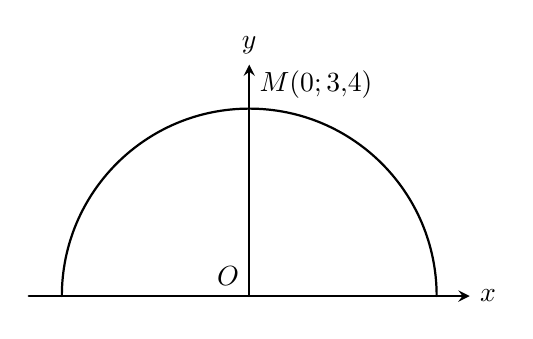
\begin{tikzpicture}[domain=0:4,line join = round, line cap = round,>=stealth,thick,scale=0.7]
					\draw[->] (-4,0) -- (4,0) node[right] {$x$};
					\draw[->] (0,0) -- (0,4.2) node[above] {$y$};
					\draw(-3.4,0) arc(-180:-360:3.4);
					\draw (0,0)node[above left]{$O$};
					\draw (0,3.4)node[above right]{$M(0;3{,}4)$};
				\end{tikzpicture}
			}
			\item \immini{
				Gọi $OABC$ là thiết diện của xe tải (Hình bên).\\
				Ta có\\
				$OB=\sqrt{OA^2+OC^2}=\sqrt{2,4^2+2,5^2} \approx 3{,}5(\mathrm{m})>R=3{,}4(\mathrm{m})$.\\
				Vậy nếu đi đúng làn đường quy định thì xe tải không thể đi qua cổng.
			}{
				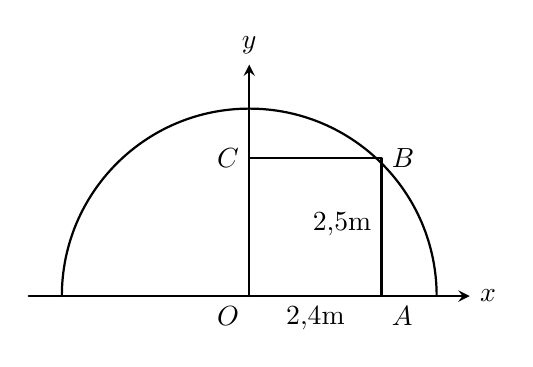
\begin{tikzpicture}[domain=0:4,line join = round, line cap = round,>=stealth,thick,scale=0.7]
					\draw[->] (-4,0) -- (4,0) node[right] {$x$};
					\draw[->] (0,0) -- (0,4.2) node[above] {$y$};
					\draw(-3.4,0) arc(-180:-360:3.4);
					\draw (0,0) node[below left]{$O$} -- (2.4,0) node[below right]{$A$}--(2.4,2.5)node[right]{$B$} --(0, 2.5)node[left]{$C$}--(0,0);
					\draw (1.2,0) node[below]{$2{,}4 \mathrm{m}$};
					\draw (2.4, 1.3) node[left]{$2{,}5\mathrm{m}$};
				\end{tikzpicture}
			}
		\end{listEX}
	}
\end{baitap}\cham{10}

\begin{baitap}
	Chuyển động của một vật thể trong khoảng thời gian 90 phút được thể hiện trong mặt phẳng toạ độ. Theo đó, tại thời điểm $t(0 \leq t \leq 90)$ vật thể ở vị trí có toạ độ $\left(1+\sin t^{\circ} ; 3+\cos t^{\circ}\right)$.
	\begin{enumEX}[a)]{1}
		\item Tìm vị trí ban đầu và vị trí kết thúc của vật thể.
		\item Tìm quỹ đạo chuyển động của vật thể.
	\end{enumEX}
	\loigiai{
		\begin{enumEX}[a)]{1}
			\item Vị trí ban đầu của vật thể là tại thời điểm $t=0$ nên tọa độ của điểm là:
			$\left(1+\sin 0^{\circ} ; 3+\cos 0^{\circ}\right)=(1 ; 4)$.
			Vị trí kết thúc của vật thể là tại thời điểm $t=90$ nên tọa độ của điểm là:
			$$
			\left(2+\sin 90^{\circ} ; 4+\cos 90^{\circ}\right)=(3 ; 4) \text {. }
			$$
			\item Gọi điểm $M(x ; y)$ thuộc vào quỹ đạo chuyển động của vật thể.
			Ta có: $x=1+\sin t^{\circ}$ và $y=3+\cos t^{\circ}$ suy ra $x-1=\sin t^{\circ}$ và $y-3=\cos t^{\circ}$
			Mà $\sin ^2 t^{\circ}+\cos ^2 t^{\circ}=1$ nên $(x-1)^2+(y-3)^2=1$.
			Vậy quỹ đạo chuyền động của vật thể là đường tròn có tâm $I(1 ; 3)$ và bán kính bằng 1 
	\end{enumEX}}
\end{baitap}\cham{10}

\begin{ex}
	\immini[thm]{Hình bên mô phỏng một trạm thu phát sóng điện thoại di động đặt ở vị trí $I$ có tọa độ $I(-2;1)$ trong mặt phẳng tọa độ (đơn vị trên hai trục là ki-lô-mét).
			\begin{enumerate}
			\item Lập phương trình đường tròn mô tả ranh giới bên ngoài của vùng phủ sóng, biết rằng trạm thu phát sóng đó đươc thiết kế với bán kính phủ sóng $3$ km.
			\item Nếu người sử dụng điện thoại ở vị trí có tọa độ $(-1;3)$ thì có thể sử dụng dịch vụ của trạm này không?
			\item Tính theo đường chim bay, xác định khoảng cách ngắn nhất để một người ở vị trí có tọa độ $(-3;4)$ di chuyển được tới vùng phủ sóng theo đơn vị ki-lô-mét (làm tròn kết quả đến hàng phần mười).
		\end{enumerate}
	}
	{
		\begin{tikzpicture}[>=stealth,line join=round,line cap=round,font=\footnotesize,scale=0.8,xscale=0.8, yscale=0.8]
			\draw[->] (-7,0)--(3,0) node[below]{$x$};
			\draw[->] (0,-3)--(0,5) node[left]{$y$};
			\coordinate (O) at (0,0);
			\coordinate (I) at (-2,1);
			\draw (I) circle(3cm);
			\draw[dashed] (-2,0)|-(0,1);
			\draw[fill=black] 
			(I) circle(1pt) node[left]{$I$}
			(-2,2) node[above]{Trạm phát sóng}
			(0,1) circle(1pt) node[above left]{$1$}
			(-2,0) circle(1pt) node[below]{$-2$}
			(0,0) circle(1pt) node[below left]{$O$}
			(1,0) circle(1pt) node[below]{$1$}
			;
		\end{tikzpicture}
	}
	\loigiai{
		\begin{enumerate}
			\item Đường tròn ranh giới có tâm $I(-2;1)$, bán kính $R=3$ có phương trình là $(C)\colon (x+2)^2+(y-1)^2=9$.
			\item Xét vị trí $A(-1;3)$, ta có $IA=\sqrt{(-1+2)^2+(3-1)^2}=\sqrt{5}<3$.\\
			Vậy người sử dụng điện thoại ở vị trí $(-1;3)$ có thể sử dụng dịch vụ của trạm này.
			\item Xét điểm $B(-3;4)$, ta có $IB=\sqrt{(-3+2)^2+(4-1)^2}=\sqrt{10}>3$.\\
			Nên điểm $B$ nằm ngoài đường tròn $(C)$.\\
			Vậy khoảng cách ngắn nhất để người đó đi đến vùng phủ sóng là $\sqrt{10}-3\approx 0{,}2$ km.
		\end{enumerate}
	}
\end{ex}
\begin{baitap}%[Tex hóa SGK CD-CT,T7/22, Đoàn Minh Tân]%[0H3T2-3]
	\immini{Ném đĩa là một môn thể thao thi đấu trong Thế vận hội Olympic mùa hè. Khi thực hiện cú ném, vận động viên thường quay lưng lại với hướng ném, sau đó xoay ngược chiều kim đồng hồ một vòng rưỡi của đường tròn để lấy đà rồi thả tay ra khỏi đĩa. Giả sử đĩa chuyển động trên một đường tròn tâm $I\left(0;\dfrac{3}{2}\right)$ bán kính $0{,}8$ trong mặt phẳng tọa độ $Oxy$ (đơn vị trên hai trục là mét). Đến điểm $M\left(\dfrac{\sqrt{39}}{10};2\right)$, đĩa được ném đi (hình bên). Trong những giây đầu tiên ngay sau khi được ném đi, quỹ đạo chuyển động của chiếc đĩa có phương trình như thế nào?
	}
	{
		\begin{tikzpicture}[>=stealth,line join=round,line cap=round,font=\footnotesize,scale=1,xscale=0.8, yscale=0.8]
			\draw[->] (-3,0)--(3,0) node[below]{$x$};
			\draw[->] (0,-1)--(0,7) node[left]{$y$};
			\coordinate (O) at (0,0);
			\coordinate (I) at (0,1.5);
			\coordinate (M) at (0.624,2);
			\coordinate (a) at ($(M)!4!-90:(I)$);
			\draw (I) circle(0.8 cm) (M)--(a);
			\draw[fill=black] 
			(I) circle(1pt) node[left]{$I$}
			(0,2) circle(1pt) node[left]{$2$}
			(M) circle(1pt) node[above]{$M$}
			(a) circle(1pt)
			($(a)+(-0.3,0.2)$) circle(1pt)
			($(a)+(-0.6,0.4)$) circle(1pt)
			($(a)+(-0.8,0.5)$) circle(1pt)
			;
		\end{tikzpicture}
	}
	\loigiai{
		Xét đường tròn $(C)$ tâm $I\left(0;\dfrac{3}{2}\right)$, bán kính $R=0{,}8$.\\
		Ta có $IM=\sqrt{\left(\dfrac{\sqrt{39}}{10}-0\right)^2+\left(2-\dfrac{3}{2}\right)^2}=0{,}8$.\\
		Suy ra điểm $M$ thuộc đường tròn tâm $I$, bán kính $R=0{,}8$.\\
		Trong những giây đầu tiên sau khi ném đi, quỹ đạo chuyển động của chiếc đĩa là một đường thẳng có phương trình là phương trình tiếp tuyến của đường tròn tại điểm $M\left(\dfrac{\sqrt{39}}{10};2\right)$
		$$\left(\dfrac{\sqrt{39}}{10}-0\right)\left(x-\dfrac{\sqrt{39}}{10}\right)+\left(2-\dfrac{3}{2}\right)(y-2)=0\Leftrightarrow\dfrac{\sqrt{39}}{10}x+\dfrac{1}{2}y+\dfrac{261}{100}=0.$$
	}
\end{baitap}\cham{27}